% !TEX program = xelatex
\documentclass[UTF8,fontset=fandol,a4paper,11pt]{ctexart}
\usepackage[margin=21mm,top=23mm,bottom=22mm,headheight=16pt]{geometry}
\usepackage{amsmath,amssymb,mathtools,bm}
\usepackage{tikz}
\usetikzlibrary{arrows.meta,calc,angles,quotes,patterns}
\usepackage{xcolor,booktabs,array,longtable,enumitem,fancyhdr,needspace}
\usepackage[unicode,hidelinks]{hyperref}
\definecolor{ink}{HTML}{24343C}
\definecolor{accent}{HTML}{166A70}
\definecolor{muted}{HTML}{65747A}
\definecolor{rulegray}{HTML}{D4DDE0}
\definecolor{warm}{HTML}{966037}
\color{ink}
\setlength{\parindent}{2em}
\setlength{\parskip}{4pt}
\linespread{1.12}
\AtBeginDocument{\setlength{\abovedisplayskip}{6pt plus 2pt minus 1pt}
\setlength{\belowdisplayskip}{6pt plus 2pt minus 1pt}
\setlength{\abovedisplayshortskip}{0pt plus 1pt}
\setlength{\belowdisplayshortskip}{4pt plus 1pt}}
\setlist[enumerate]{label=(\arabic*),leftmargin=2.3em,itemsep=3pt,topsep=4pt}
\setlist[itemize]{leftmargin=2em,itemsep=2pt,topsep=4pt}
\allowdisplaybreaks[1]
\setlength{\emergencystretch}{2em}
\setcounter{secnumdepth}{0}
\providecommand{\tightlist}{\setlength{\itemsep}{0pt}\setlength{\parskip}{0pt}}
\ctexset{section={format=\Large\bfseries\color{accent},beforeskip=10pt,afterskip=9pt},
subsection={format=\normalsize\bfseries\color{accent},beforeskip=10pt,afterskip=4pt},
subsubsection={format=\normalsize\bfseries,beforeskip=8pt,afterskip=3pt}}
\pagestyle{fancy}
\fancyhf{}
\fancyhead[L]{\small\color{muted}物理学难题集萃}
% 页眉仅保留书名；版本名称只在封面显示。
\fancyfoot[L]{\small\color{muted}\chapterlabel}
\fancyfoot[R]{\small\thepage}
\renewcommand{\headrulewidth}{0.4pt}
\renewcommand{\footrulewidth}{0pt}
\newcommand{\dd}{\mathop{}\!\mathrm{d}}
\newcommand{\vect}[1]{\bm{#1}}
\newcommand{\tagline}[1]{\noindent{\small\color{muted}#1}\par}
\newcommand{\result}[1]{\begin{equation*}\boxed{#1}\end{equation*}}
\newcommand{\figcaption}[1]{\par\vspace{2pt}{\small\color{muted}#1}\par}
\newcommand{\teach}[2]{\Needspace{4\baselineskip}\subsection*{讲解要点与追问}#1\par\smallskip\noindent\textbf{追问：}#2\par}
\newcommand{\workarea}{\par\vspace{7mm}\noindent{\small\color{muted}作答区}\par\vspace{4mm}
\noindent\textcolor{rulegray}{\rule{\linewidth}{0.3pt}}\par\vspace{16mm}
\noindent\textcolor{rulegray}{\rule{\linewidth}{0.3pt}}\par\vspace{16mm}
\noindent\textcolor{rulegray}{\rule{\linewidth}{0.3pt}}\par\vspace{16mm}
\noindent\textcolor{rulegray}{\rule{\linewidth}{0.3pt}}}
\tikzset{axis/.style={-{Stealth[length=2mm]},thin,color=muted},
motion/.style={-{Stealth[length=2.3mm]},thick,color=accent},
force/.style={-{Stealth[length=2.3mm]},thick,color=warm},
traj/.style={thick,color=accent},guide/.style={dashed,thin,color=muted},
object/.style={thick,color=ink},every node/.style={font=\small}}\widowpenalty=10000\clubpenalty=10000\displaywidowpenalty=10000\newcommand{\chapterlabel}{力学试题（一）}







\hypersetup{pdftitle={力学试题一 力学试题（一）·学生版},pdfauthor={}}

\begin{document}\pdfbookmark[0]{力学试题一 力学试题（一）}{cover}

\thispagestyle{empty}\vspace*{22mm}

\noindent{\Huge\bfseries 物理学难题集萃}\par\vspace{10mm}

\noindent{\LARGE 力学试题一}\par\vspace{6mm}

\noindent{\LARGE 力学试题（一）}\par\vspace{12mm}

\noindent{\Large\color{accent}学生版}\par\vspace{9mm}

\noindent\textcolor{accent}{\rule{\linewidth}{1pt}}\par\vspace{9mm}

\noindent 第1--6题\par\vfill\clearpage

\pdfbookmark[1]{题目目录}{contents}\section*{题目目录}

\begin{longtable}{@{}r p{113mm} r@{}}\toprule 题号 & 题目 & 页码\\\midrule

\hyperref[q:1]{1} & \hyperref[q:1]{飞行中拦截与最小发射速度} & \pageref{q:1} \\

\hyperref[q:2]{2} & \hyperref[q:2]{可移动圆环内小球的轨迹与曲率} & \pageref{q:2} \\

\hyperref[q:3]{3} & \hyperref[q:3]{螺旋槽内下滑与圆筒的平移、自转} & \pageref{q:3} \\

\hyperref[q:4]{4} & \hyperref[q:4]{弹出小球与自由细杆端点再次相遇} & \pageref{q:4} \\

\hyperref[q:5]{5} & \hyperref[q:5]{切向减速后的陨石近地点} & \pageref{q:5} \\

\hyperref[q:6]{6} & \hyperref[q:6]{绳杆受冲量后的初动与摆角条件} & \pageref{q:6} \\

\bottomrule\end{longtable}

\clearpage

\pdfbookmark[2]{第 1 题 飞行中拦截与最小发射速度}{q1}

\section*{第 1 题\quad 飞行中拦截与最小发射速度}\label{q:1}


轰炸机以水平速度$v_1>0$在高度$H$匀速飞行，投下炸弹，目标在其前方地面上。忽略空气阻力，取重力加速度为$g$。
\begin{enumerate}
\item 为使炸弹命中目标，应在离目标多远的水平位置投弹？
\item 炮位在目标后方、沿飞机飞行方向量距目标为$D\ge0$。飞机投弹的同时，高射炮发射炮弹。求使炮弹在炸弹落地前击中它所需发射速度的最小值；同时说明最小值的可取条件与速度下界。
\item 求相应的发射方向，并说明相遇时刻是否满足“飞行中”的要求。
\end{enumerate}
飞机、炮位与目标在同一竖直平面；两弹均视为质点，发射方向可在该平面内选取。发射角$\alpha$从水平正向量起，向上为正。


\begin{center}\begin{minipage}{.98\linewidth}\centering
\begin{tikzpicture}[scale=.9,transform shape]
\draw[object] (0.00000,0.00000)--(8.20000,0.00000);\fill (0.00000,4.00000) circle(.035);\node[above left] at (0.00000,4.00000) {投弹点};\fill (0.00000,0.00000) circle(.035);\node[below] at (0.00000,0.00000) {$O$};\fill (8.00000,0.00000) circle(.035);\node[below right] at (8.00000,0.00000) {目标 $G$};\fill (4.00000,0.00000) circle(.035);\node[above] at (4.00000,0.00000) {炮位 $P$};\draw[motion] (0.00000,4.00000)--(1.60000,4.00000);\node[above] at (0.80000,4.10000) {$v_1$};\draw[<->,thin,color=muted] (-0.70000,0.00000)--(-0.70000,4.00000);\node[left] at (-0.70000,2.00000) {$H$};\draw[<->,thin,color=muted] (0.00000,-1.00000)--(8.00000,-1.00000);\node[below] at (4.00000,-1.00000) {$L$};\draw[<->,thin,color=muted] (4.00000,-2.00000)--(8.00000,-2.00000);\node[below] at (6.00000,-2.00000) {$D$};
\end{tikzpicture}
\figcaption{图力试1.1\quad 投弹点、炮位与目标的水平位置；D允许取零。}
\end{minipage}\end{center}

\workarea

\clearpage

\pdfbookmark[2]{第 2 题 可移动圆环内小球的轨迹与曲率}{q2}

\section*{第 2 题\quad 可移动圆环内小球的轨迹与曲率}\label{q:2}


半径为$R$的竖直空心圆环固定在滑块上，环和滑块总质量为$M$，可在光滑水平地面上平移而不转动。质量为$m$的小球视为质点，可在环内的光滑管道中运动。

开始时环与球都静止，球在最高点。用极小扰动使球向右下滑，讨论扰动趋零时的轨迹。以初始环心$O$为地面坐标原点，水平向右为$x$，竖直向上为$y$。求：
\begin{enumerate}
\item 小球相对地面的轨迹方程。
\item 小球经过圆环右侧点$A$及最低点$B$时，地面轨迹的曲率半径。要求用受力与相对运动说明，而不只引用椭圆曲率公式。
\end{enumerate}


\begin{center}\begin{minipage}{.98\linewidth}\centering
\begin{tikzpicture}[scale=.9,transform shape]
\draw[object] (0.00000,0.00000) circle(3.00000);\draw[object] (-1.50000,-3.10000)--(1.50000,-3.10000)--(1.50000,-3.50000)--(-1.50000,-3.50000)--(-1.50000,-3.10000);\draw[object] (-2.00000,-3.65000)--(2.00000,-3.65000);\draw[object] (-1.00000,-2.82843)--(-1.00000,-3.10000);\draw[object] (1.00000,-2.82843)--(1.00000,-3.10000);\fill (0.00000,3.00000) circle(.035);\node[above] at (0.00000,3.00000) {$m$};\fill (3.00000,0.00000) circle(.035);\node[right] at (3.00000,0.00000) {$A$};\fill (0.00000,-3.00000) circle(.035);\node[above right] at (0.00000,-3.00000) {$B$};\fill (0.00000,0.00000) circle(.035);\node[above left] at (0.00000,0.00000) {$O$};\draw[<->,thin,color=muted] (0.00000,-0.40000)--(3.00000,-0.40000);\node[below] at (1.50000,-0.40000) {$R$};\node[below] at (0.00000,-4.00000) {环与滑块总质量 $M$};
\end{tikzpicture}
\figcaption{图力试1.2\quad 球从环顶向右微扰，A为相对圆的右侧点，B为底点。}
\end{minipage}\end{center}

\workarea

\clearpage

\pdfbookmark[2]{第 3 题 螺旋槽内下滑与圆筒的平移、自转}{q3}

\section*{第 3 题\quad 螺旋槽内下滑与圆筒的平移、自转}\label{q:3}


质量为$M$、半径为$R$的均匀薄壁圆筒竖直放在光滑水平面上，可水平平移并绕竖直轴自转，保持竖直而不倾倒。筒内壁有一条光滑螺旋槽，筒高$h$恰等于螺距，即沿槽绕筒一周恰从顶端到达底端。小球质量为$m$，从槽顶与圆筒一同静止开始下滑。
\begin{enumerate}
\item 说明下滑过程中圆筒轴线的水平运动与圆筒自转。
\item 求小球从槽顶到槽底相对地面走过的总路程。
\end{enumerate}
圆筒绕自身竖直轴的转动惯量为$I=MR^2$。忽略摩擦和小球尺寸。


\begin{center}\begin{minipage}{.98\linewidth}\centering
\begin{tikzpicture}[scale=.9,transform shape]
\draw[object] plot coordinates {(2.00000,0.00000) (1.99822,0.01897) (1.99289,0.03791) (1.98402,0.05678) (1.97162,0.07554) (1.95571,0.09418) (1.93632,0.11265) (1.91350,0.13091) (1.88727,0.14895) (1.85768,0.16671) (1.82480,0.18419) (1.78866,0.20133) (1.74935,0.21812) (1.70693,0.23452) (1.66147,0.25050) (1.61306,0.26604) (1.56178,0.28110) (1.50773,0.29566) (1.45099,0.30970) (1.39167,0.32319) (1.32988,0.33610) (1.26573,0.34842) (1.19932,0.36011) (1.13078,0.37117) (1.06024,0.38157) (0.98780,0.39128) (0.91361,0.40030) (0.83780,0.40861) (0.76049,0.41620) (0.68184,0.42304) (0.60197,0.42913) (0.52103,0.43446) (0.43917,0.43902) (0.35652,0.44279) (0.27324,0.44578) (0.18948,0.44798) (0.10537,0.44937) (0.02108,0.44997) (-0.06324,0.44977) (-0.14746,0.44878) (-0.23141,0.44698) (-0.31495,0.44439) (-0.39793,0.44100) (-0.48021,0.43684) (-0.56163,0.43189) (-0.64205,0.42618) (-0.72133,0.41971) (-0.79932,0.41250) (-0.87590,0.40455) (-0.95092,0.39588) (-1.02425,0.38651) (-1.09575,0.37645) (-1.16531,0.36572) (-1.23280,0.35435) (-1.29809,0.34234) (-1.36108,0.32972) (-1.42165,0.31652) (-1.47969,0.30275) (-1.53510,0.28845) (-1.58778,0.27363) (-1.63763,0.25833) (-1.68458,0.24256) (-1.72853,0.22637) (-1.76940,0.20977) (-1.80713,0.19280) (-1.84165,0.17549) (-1.87289,0.15786) (-1.90081,0.13996) (-1.92534,0.12181) (-1.94645,0.10344) (-1.96410,0.08488) (-1.97826,0.06618) (-1.98890,0.04735) (-1.99600,0.02845) (-1.99956,0.00949) (-1.99956,-0.00949) (-1.99600,-0.02845) (-1.98890,-0.04735) (-1.97826,-0.06618) (-1.96410,-0.08488) (-1.94645,-0.10344) (-1.92534,-0.12181) (-1.90081,-0.13996) (-1.87289,-0.15786) (-1.84165,-0.17549) (-1.80713,-0.19280) (-1.76940,-0.20977) (-1.72853,-0.22637) (-1.68458,-0.24256) (-1.63763,-0.25833) (-1.58778,-0.27363) (-1.53510,-0.28845) (-1.47969,-0.30275) (-1.42165,-0.31652) (-1.36108,-0.32972) (-1.29809,-0.34234) (-1.23280,-0.35435) (-1.16531,-0.36572) (-1.09575,-0.37645) (-1.02425,-0.38651) (-0.95092,-0.39588) (-0.87590,-0.40455) (-0.79932,-0.41250) (-0.72133,-0.41971) (-0.64205,-0.42618) (-0.56163,-0.43189) (-0.48021,-0.43684) (-0.39793,-0.44100) (-0.31495,-0.44439) (-0.23141,-0.44698) (-0.14746,-0.44878) (-0.06324,-0.44977) (0.02108,-0.44997) (0.10537,-0.44937) (0.18948,-0.44798) (0.27324,-0.44578) (0.35652,-0.44279) (0.43917,-0.43902) (0.52103,-0.43446) (0.60197,-0.42913) (0.68184,-0.42304) (0.76049,-0.41620) (0.83780,-0.40861) (0.91361,-0.40030) (0.98780,-0.39128) (1.06024,-0.38157) (1.13078,-0.37117) (1.19932,-0.36011) (1.26573,-0.34842) (1.32988,-0.33610) (1.39167,-0.32319) (1.45099,-0.30970) (1.50773,-0.29566) (1.56178,-0.28110) (1.61306,-0.26604) (1.66147,-0.25050) (1.70693,-0.23452) (1.74935,-0.21812) (1.78866,-0.20133) (1.82480,-0.18419) (1.85768,-0.16671) (1.88727,-0.14895) (1.91350,-0.13091) (1.93632,-0.11265) (1.95571,-0.09418) (1.97162,-0.07554) (1.98402,-0.05678) (1.99289,-0.03791) (1.99822,-0.01897) (2.00000,-0.00000)};\draw[object] plot coordinates {(2.00000,5.00000) (1.99822,5.01897) (1.99289,5.03791) (1.98402,5.05678) (1.97162,5.07554) (1.95571,5.09418) (1.93632,5.11265) (1.91350,5.13091) (1.88727,5.14895) (1.85768,5.16671) (1.82480,5.18419) (1.78866,5.20133) (1.74935,5.21812) (1.70693,5.23452) (1.66147,5.25050) (1.61306,5.26604) (1.56178,5.28110) (1.50773,5.29566) (1.45099,5.30970) (1.39167,5.32319) (1.32988,5.33610) (1.26573,5.34842) (1.19932,5.36011) (1.13078,5.37117) (1.06024,5.38157) (0.98780,5.39128) (0.91361,5.40030) (0.83780,5.40861) (0.76049,5.41620) (0.68184,5.42304) (0.60197,5.42913) (0.52103,5.43446) (0.43917,5.43902) (0.35652,5.44279) (0.27324,5.44578) (0.18948,5.44798) (0.10537,5.44937) (0.02108,5.44997) (-0.06324,5.44977) (-0.14746,5.44878) (-0.23141,5.44698) (-0.31495,5.44439) (-0.39793,5.44100) (-0.48021,5.43684) (-0.56163,5.43189) (-0.64205,5.42618) (-0.72133,5.41971) (-0.79932,5.41250) (-0.87590,5.40455) (-0.95092,5.39588) (-1.02425,5.38651) (-1.09575,5.37645) (-1.16531,5.36572) (-1.23280,5.35435) (-1.29809,5.34234) (-1.36108,5.32972) (-1.42165,5.31652) (-1.47969,5.30275) (-1.53510,5.28845) (-1.58778,5.27363) (-1.63763,5.25833) (-1.68458,5.24256) (-1.72853,5.22637) (-1.76940,5.20977) (-1.80713,5.19280) (-1.84165,5.17549) (-1.87289,5.15786) (-1.90081,5.13996) (-1.92534,5.12181) (-1.94645,5.10344) (-1.96410,5.08488) (-1.97826,5.06618) (-1.98890,5.04735) (-1.99600,5.02845) (-1.99956,5.00949) (-1.99956,4.99051) (-1.99600,4.97155) (-1.98890,4.95265) (-1.97826,4.93382) (-1.96410,4.91512) (-1.94645,4.89656) (-1.92534,4.87819) (-1.90081,4.86004) (-1.87289,4.84214) (-1.84165,4.82451) (-1.80713,4.80720) (-1.76940,4.79023) (-1.72853,4.77363) (-1.68458,4.75744) (-1.63763,4.74167) (-1.58778,4.72637) (-1.53510,4.71155) (-1.47969,4.69725) (-1.42165,4.68348) (-1.36108,4.67028) (-1.29809,4.65766) (-1.23280,4.64565) (-1.16531,4.63428) (-1.09575,4.62355) (-1.02425,4.61349) (-0.95092,4.60412) (-0.87590,4.59545) (-0.79932,4.58750) (-0.72133,4.58029) (-0.64205,4.57382) (-0.56163,4.56811) (-0.48021,4.56316) (-0.39793,4.55900) (-0.31495,4.55561) (-0.23141,4.55302) (-0.14746,4.55122) (-0.06324,4.55023) (0.02108,4.55003) (0.10537,4.55063) (0.18948,4.55202) (0.27324,4.55422) (0.35652,4.55721) (0.43917,4.56098) (0.52103,4.56554) (0.60197,4.57087) (0.68184,4.57696) (0.76049,4.58380) (0.83780,4.59139) (0.91361,4.59970) (0.98780,4.60872) (1.06024,4.61843) (1.13078,4.62883) (1.19932,4.63989) (1.26573,4.65158) (1.32988,4.66390) (1.39167,4.67681) (1.45099,4.69030) (1.50773,4.70434) (1.56178,4.71890) (1.61306,4.73396) (1.66147,4.74950) (1.70693,4.76548) (1.74935,4.78188) (1.78866,4.79867) (1.82480,4.81581) (1.85768,4.83329) (1.88727,4.85105) (1.91350,4.86909) (1.93632,4.88735) (1.95571,4.90582) (1.97162,4.92446) (1.98402,4.94322) (1.99289,4.96209) (1.99822,4.98103) (2.00000,5.00000)};\draw[object] (-2.00000,0.00000)--(-2.00000,5.00000);\draw[object] (2.00000,0.00000)--(2.00000,5.00000);\draw[traj] plot coordinates {(2.00000,5.00000) (1.99918,4.99008) (1.99671,4.98015) (1.99260,4.97019) (1.98684,4.96021) (1.97946,4.95018) (1.97044,4.94010) (1.95980,4.92995) (1.94755,4.91973) (1.93370,4.90943) (1.91825,4.89903) (1.90122,4.88853) (1.88263,4.87791) (1.86250,4.86717) (1.84082,4.85629) (1.81764,4.84527) (1.79295,4.83409) (1.76679,4.82275) (1.73918,4.81124) (1.71013,4.79954) (1.67968,4.78765) (1.64785,4.77556) (1.61465,4.76326) (1.58013,4.75075) (1.54431,4.73800) (1.50722,4.72502) (1.46889,4.71179) (1.42935,4.69832) (1.38863,4.68458) (1.34677,4.67058) (1.30380,4.65631) (1.25976,4.64175) (1.21468,4.62691) (1.16860,4.61177) (1.12156,4.59633) (1.07359,4.58058) (1.02474,4.56453) (0.97505,4.54815) (0.92456,4.53145) (0.87330,4.51442) (0.82133,4.49706) (0.76868,4.47936) (0.71540,4.46132) (0.66153,4.44294) (0.60711,4.42420) (0.55219,4.40511) (0.49682,4.38567) (0.44105,4.36586) (0.38490,4.34570) (0.32844,4.32517) (0.27172,4.30428) (0.21476,4.28301) (0.15763,4.26139) (0.10037,4.23939) (0.04303,4.21702) (-0.01435,4.19428) (-0.07171,4.17117) (-0.12902,4.14769) (-0.18622,4.12384) (-0.24326,4.09963) (-0.30011,4.07504) (-0.35671,4.05009) (-0.41302,4.02478) (-0.46898,3.99910) (-0.52456,3.97306) (-0.57971,3.94666) (-0.63438,3.91991) (-0.68853,3.89281) (-0.74211,3.86536) (-0.79509,3.83757) (-0.84740,3.80944) (-0.89902,3.78097) (-0.94990,3.75217) (-1.00000,3.72304) (-1.04927,3.69360) (-1.09769,3.66384) (-1.14519,3.63377) (-1.19176,3.60339) (-1.23734,3.57272) (-1.28191,3.54176) (-1.32542,3.51051) (-1.36784,3.47899) (-1.40913,3.44719) (-1.44927,3.41513) (-1.48821,3.38282) (-1.52592,3.35026) (-1.56238,3.31746) (-1.59756,3.28443) (-1.63142,3.25118) (-1.66393,3.21771) (-1.69508,3.18403) (-1.72483,3.15016) (-1.75317,3.11611) (-1.78006,3.08187) (-1.80548,3.04747) (-1.82942,3.01290) (-1.85185,2.97819) (-1.87276,2.94333) (-1.89212,2.90835) (-1.90993,2.87325) (-1.92617,2.83803) (-1.94082,2.80272) (-1.95388,2.76732) (-1.96532,2.73184) (-1.97515,2.69629) (-1.98335,2.66068) (-1.98993,2.62502) (-1.99486,2.58933) (-1.99815,2.55361) (-1.99979,2.51787) (-1.99979,2.48213) (-1.99815,2.44639) (-1.99486,2.41067) (-1.98993,2.37498) (-1.98335,2.33932) (-1.97515,2.30371) (-1.96532,2.26816) (-1.95388,2.23268) (-1.94082,2.19728) (-1.92617,2.16197) (-1.90993,2.12675) (-1.89212,2.09165) (-1.87276,2.05667) (-1.85185,2.02181) (-1.82942,1.98710) (-1.80548,1.95253) (-1.78006,1.91813) (-1.75317,1.88389) (-1.72483,1.84984) (-1.69508,1.81597) (-1.66393,1.78229) (-1.63142,1.74882) (-1.59756,1.71557) (-1.56238,1.68254) (-1.52592,1.64974) (-1.48821,1.61718) (-1.44927,1.58487) (-1.40913,1.55281) (-1.36784,1.52101) (-1.32542,1.48949) (-1.28191,1.45824) (-1.23734,1.42728) (-1.19176,1.39661) (-1.14519,1.36623) (-1.09769,1.33616) (-1.04927,1.30640) (-1.00000,1.27696) (-0.94990,1.24783) (-0.89902,1.21903) (-0.84740,1.19056) (-0.79509,1.16243) (-0.74211,1.13464) (-0.68853,1.10719) (-0.63438,1.08009) (-0.57971,1.05334) (-0.52456,1.02694) (-0.46898,1.00090) (-0.41302,0.97522) (-0.35671,0.94991) (-0.30011,0.92496) (-0.24326,0.90037) (-0.18622,0.87616) (-0.12902,0.85231) (-0.07171,0.82883) (-0.01435,0.80572) (0.04303,0.78298) (0.10037,0.76061) (0.15763,0.73861) (0.21476,0.71699) (0.27172,0.69572) (0.32844,0.67483) (0.38490,0.65430) (0.44105,0.63414) (0.49682,0.61433) (0.55219,0.59489) (0.60711,0.57580) (0.66153,0.55706) (0.71540,0.53868) (0.76868,0.52064) (0.82133,0.50294) (0.87330,0.48558) (0.92456,0.46855) (0.97505,0.45185) (1.02474,0.43547) (1.07359,0.41942) (1.12156,0.40367) (1.16860,0.38823) (1.21468,0.37309) (1.25976,0.35825) (1.30380,0.34369) (1.34677,0.32942) (1.38863,0.31542) (1.42935,0.30168) (1.46889,0.28821) (1.50722,0.27498) (1.54431,0.26200) (1.58013,0.24925) (1.61465,0.23674) (1.64785,0.22444) (1.67968,0.21235) (1.71013,0.20046) (1.73918,0.18876) (1.76679,0.17725) (1.79295,0.16591) (1.81764,0.15473) (1.84082,0.14371) (1.86250,0.13283) (1.88263,0.12209) (1.90122,0.11147) (1.91825,0.10097) (1.93370,0.09057) (1.94755,0.08027) (1.95980,0.07005) (1.97044,0.05990) (1.97946,0.04982) (1.98684,0.03979) (1.99260,0.02981) (1.99671,0.01985) (1.99918,0.00992) (2.00000,-0.00000)};\fill (2.00000,5.00000) circle(.035);\node[above right] at (2.00000,5.00000) {$m$};\draw[<->,thin,color=muted] (3.00000,0.00000)--(3.00000,5.00000);\node[right] at (3.00000,2.50000) {$h$};\draw[<->,thin,color=muted] (0.00000,-1.00000)--(2.00000,-1.00000);\node[below] at (1.00000,-1.00000) {$R$};\node[above] at (0.00000,6.00000) {薄壁圆筒 $M$；螺旋槽一周};
\end{tikzpicture}
\figcaption{图力试1.3\quad 可平移、自转的圆筒及固定在筒壁上的一周槽。}
\end{minipage}\end{center}

\workarea

\clearpage

\pdfbookmark[2]{第 4 题 弹出小球与自由细杆端点再次相遇}{q4}

\section*{第 4 题\quad 弹出小球与自由细杆端点再次相遇}\label{q:4}


质量为$M$、长度为$l$的均匀细杆$AB$静止在光滑水平面上。$B$端的轻弹簧将质量为$m$的小球斜向弹出，弹出后小球的地面速度大小为$v$，与从$B$指向$A$的方向夹角为$\varphi$，$0<\varphi<\pi/2$。

要求小球自由运动后恰与杆的$A$端相遇，且相遇前细杆的转角不超过$\pi$。求质量比$\gamma=M/m$与发射角$\varphi$的关系及其允许范围。忽略球与杆的厚度、摩擦和弹簧质量，弹出后到再次相遇前球与杆无相互作用。


\begin{center}\begin{minipage}{.98\linewidth}\centering
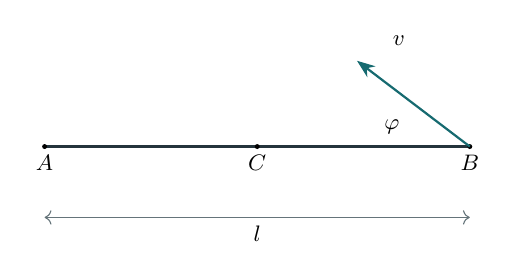
\begin{tikzpicture}[scale=.9,transform shape]
\draw[object] (-3.00000,0.00000)--(3.00000,0.00000);\fill (-3.00000,0.00000) circle(.035);\node[below] at (-3.00000,0.00000) {$A$};\fill (0.00000,0.00000) circle(.035);\node[below] at (0.00000,0.00000) {$C$};\fill (3.00000,0.00000) circle(.035);\node[below] at (3.00000,0.00000) {$B$};\draw[motion] (3.00000,0.00000)--(1.40783,1.21037);\node[above] at (2.00000,1.30000) {$v$};\node[above] at (1.90000,0.05000) {$\varphi$};\draw[<->,thin,color=muted] (-3.00000,-1.00000)--(3.00000,-1.00000);\node[below] at (0.00000,-1.00000) {$l$};
\end{tikzpicture}
\figcaption{图力试1.4\quad 斜向发射后，球和杆质心沿相反方向平移。}
\end{minipage}\end{center}

\workarea

\clearpage

\pdfbookmark[2]{第 5 题 切向减速后的陨石近地点}{q5}

\section*{第 5 题\quad 切向减速后的陨石近地点}\label{q:5}


一块陨石在距地表高度$h=4.2\times10^3\,\mathrm{km}$的圆轨道上绕地球运动，突然与一块小得多的陨石正碰，碰后动能减少2\%。把碰撞视为瞬时过程，假定大陨石质量不变，运动方向不变，随后只受地球引力。

求碰撞后陨石离地心的最小距离。地球半径$R_E=6.4\times10^3\,\mathrm{km}$；引力按球对称处理，忽略大气阻力。


\begin{center}\begin{minipage}{.98\linewidth}\centering
\begin{tikzpicture}[scale=.9,transform shape]
\draw[object] (0,0) circle(1.8113208);
\node at (0,0) {地球};\draw[guide] (0,0) circle(3);
\fill (3,0) circle(.04) node[right] {$A$碰撞};\draw[motion] (3,0)--(3,1.4) node[right] {$v_0\to v_+$};
\draw[<->,thin,color=muted] (0,-2.4)--(3,-2.4) node[midway,below] {$r_0=R_E+h$};
\end{tikzpicture}
\figcaption{图力试1.5\quad 地球与圆轨道半径按题设比例绘制，碰撞点速度沿切线减小}
\end{minipage}\end{center}

\workarea

\clearpage

\pdfbookmark[2]{第 6 题 绳杆受冲量后的初动与摆角条件}{q6}

\section*{第 6 题\quad 绳杆受冲量后的初动与摆角条件}\label{q:6}


均匀细杆质量为$M$、长度为$2L$，由长为$l$的轻绳竖直悬挂，绳上端固定在$P$，下端接杆的上端$A$。系统起初静止。给杆下端$B$一个水平向右、持续时间极短的冲量$J$。
\begin{enumerate}
\item 画出刚开始运动时绳与杆的偏转方向。
\item 求冲量结束瞬间绳角速度$\dot\theta(0^+)$与杆角速度$\dot\varphi(0^+)$。两角都从竖直向下方向量起，向右偏为正。
\item 建立摆角与能量的关系，说明在所谓“最大摆角”时可使用什么条件；区分单个角达到极值和绳、杆同时瞬时静止。
\end{enumerate}
杆可绕绳杆连接点在竖直平面内摆动，忽略阻力。涉及后续约束运动的公式用于绳保持张紧的阶段。


\begin{center}\begin{minipage}{.98\linewidth}\centering
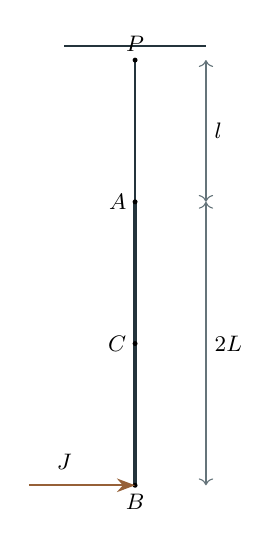
\begin{tikzpicture}[scale=.9,transform shape]
\draw[object] (-1.00000,0.20000)--(1.00000,0.20000);\draw[object] (0.00000,0.00000)--(0.00000,-2.00000);\draw[very thick,color=ink] (0.00000,-2.00000)--(0.00000,-6.00000);\fill (0.00000,0.00000) circle(.035);\node[above] at (0.00000,0.00000) {$P$};\fill (0.00000,-2.00000) circle(.035);\node[left] at (0.00000,-2.00000) {$A$};\fill (0.00000,-4.00000) circle(.035);\node[left] at (0.00000,-4.00000) {$C$};\fill (0.00000,-6.00000) circle(.035);\node[below] at (0.00000,-6.00000) {$B$};\draw[force] (-1.50000,-6.00000)--(0.00000,-6.00000);\node[above] at (-1.00000,-5.90000) {$J$};\draw[<->,thin,color=muted] (1.00000,0.00000)--(1.00000,-2.00000);\node[right] at (1.00000,-1.00000) {$l$};\draw[<->,thin,color=muted] (1.00000,-2.00000)--(1.00000,-6.00000);\node[right] at (1.00000,-4.00000) {$2L$};
\end{tikzpicture}
\figcaption{图力试1.6\quad 竖直绳杆，水平冲量施加在杆下端B。}
\end{minipage}\end{center}

\workarea

\end{document}
